% Use a modified ACM conference proceedings template
\documentclass[sigconf]{acmart}
% Disable some elements from ACM template
\setcopyright{none}
\settopmatter{printacmref=false,printfolios=false}

\usepackage{booktabs} % For formal tables
\usepackage[ruled,vlined]{algorithm2e}
\usepackage{amsmath} % for writing algorithms

% OWN COMMANDS
\newcommand{\todo}[1]{{\color{red}{#1}}}

% VARIABLES
\usepackage{xspace} % allows \commmand instead of \command{} with correct space afterwards
\newcommand{\VNumSimulations}{20\xspace}

\usepackage{cleveref}

\begin{document}
    \title{On Trust and Prosociality}

    \author{Fatjon Zogaj}\affiliation{}
    \email{fzogaj@student.ethz.ch}

    \author{Rafael Sterzinger}\affiliation{}
    \email{rsterzinger@student.ethz.ch}

    \begin{abstract}
        \todo{Briefly summarize your report here. This should include a description of the task you are solving, a summary of how you approach the task (i.e. your method), as well as a preview of the central result. The abstract should be short, i.e. 4-5 sentences. The rest of this template outlines a rough structure how you \emph{can} organize your report. It mentions all the components we would typically expect. It is a good idea to adhere these guidelines, but they are not binding, i.e., you are free to re-organize your report as you see fit.}
    \end{abstract}

    \maketitle


    \section{Introduction}
    \todo{In this section, introduce the task in a bit more detail. In the first paragraph, try to answer why the task is of interest at all and what makes it challenging. You may also discuss some related work here. For example, you can summarize how other researchers have addressed the problem and what might be the disadvantages of these works.

    In the second half of the introduction, describe your method. This should be more detailed than in the abstract. You can talk about how your method relates to existing work (e.g. it is a combination or extension of existing methods, what other papers were you inspired by, etc.). You should also state the central result here, and the key insight that made it possible to achieve this result.
    }

    How Did Cooperative Behavior Evolve? One of 25 top unsolved puzzles according to \citeauthor{noauthor_125th_nodate}.

    overview on mechanism of cooperation
    Mechanism for Altruism, Spite, Reciprocity, and Greanbeard.\cite{west_altruism_2010}


    connection from image scoringn to greenbeards/kin selection
    Probably important paper to our topic.\cite{roberts_kin_2019}

    key question of paper
    How does missinformation affect fitness? \cite{wallace_misinformation_1973}
    Very good related literature
%https://www.biorxiv.org/content/10.1101/2019.12.11.872937v1.full#F1


    \section{Related Work}
    \todo{
    This section is optional and it is fine to leave it out completely. While the most relevant papers should be discussed adequately somewhere (e.g. in the introduction), we do not expect you to give a complete overview of related work. Nonetheless, if you would like to do so, this would be the place to do it.

    Generally, use the \texttt{{\char'134}cite} command to cite other works, e.g. \cite{Douglass98,Harel79}. To add a new reference, you need to add a bibtex entry to the bibliography file, in this case \texttt{bibliography.bib}.

    }

    \subsection{Homo Socialis and Homo Economicus}\cite{helbing_homo_2019}
    \todo{chapter on cooperation (direct fitness/indirect fitness)\cite{gardner_theory_2009} probably more relevant}


    \subsection{Kin Selection}

    \subsection{Indirect Reciprocity}

    \subsection{Greenbeard Phenomenon}

    \section{Hypothesis}



    \section{Method}
    \todo{
    This section should describe the method of your \emph{final} submission in detail. This includes things you did with the data (e.g. preprocessing, augmentations, changes of representation, etc.) and the actual definition of your model. Sometimes it is fine to describe a model in text or math only, sometimes it is better to create an overview figure. Either way, after reading this section, a reader should be able to implement your architecture.
    If you have enough space, you may list hyperparameter values in an ``Implementation Details'' paragraph. Otherwise list them in the README of your code repo.
    }

    As our first step, we create an environment so that our population neither goes extinct, nor explodes in size within the 1000 day timeframe we have set.
    As can be seen in \Cref{fig:stable_pop} averaging over \VNumSimulations runs, the starting population of 100 stays roughly the same.
    \todo{Info about params}

    \begin{figure}
        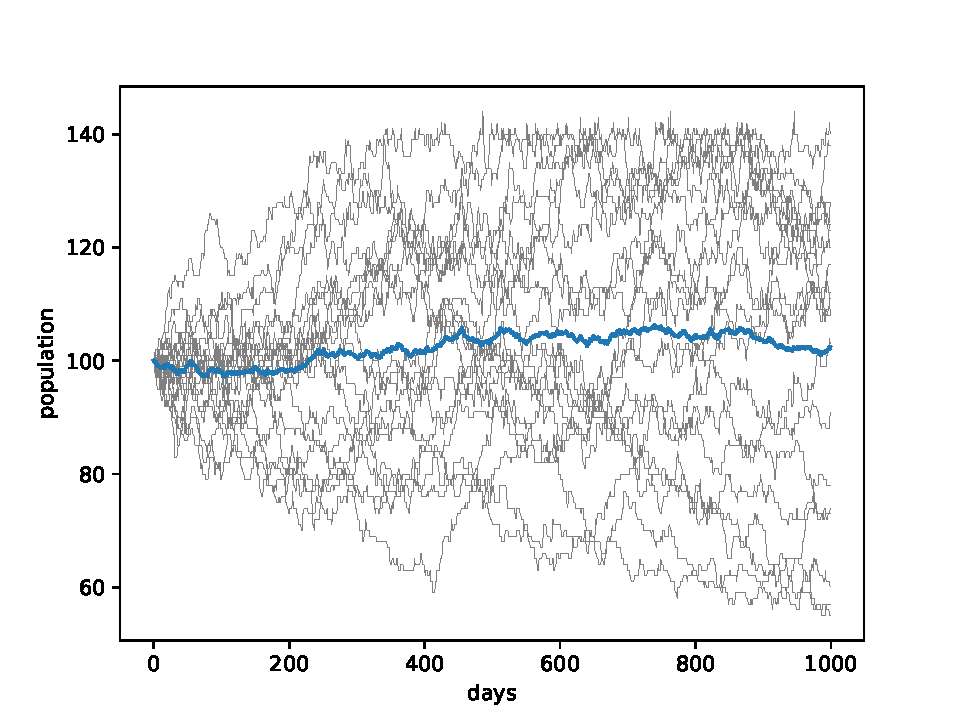
\includegraphics[width=\columnwidth]{figures/stable_population}
        \caption{While there are big deviations, on average the population stays roughly the same.
        Visualized are \VNumSimulations random runs in light grey and their average in blue. }
        \label{fig:stable_pop}
    \end{figure}


    \section{Evaluation}
    \todo{
    In the evaluation section you should describe the experiments that support the claims of the story of your report. For example, if you previously said ``We propose to combine model A with component B which leads to improved accuracy.'' you should back this up with experimental evidence here. Typically, this means that you should show the performance of model A with and without component B. May be your method warrants other kinds of such ablation studies, which you might include and describe here.

    }


    \section{Discussion}
    \todo{
    Sometimes you might have had a great idea, but it did not pan out. Since we want to encourage novelty, such failed attempts should also go into the report. This section is a suitable place to discuss this. If you can, do not just list failed attempts, but actually \emph{discuss} them, i.e., provide an intuition why you think they failed or what the problem is that prevented them from performing better. It is much better to describe one failed attempt and discuss it in-depth than just listing four failed models without any explanation.

    If you do not have failed attempts that would warrant their own section, this is perfectly fine. You may discuss the experiments from the previous section here, or if you prefer to have the discussion the evaluation section directly, feel free to omit this section entirely.

    }


    \section{Conclusion}
    \todo{
    Conclude your report with a brief summary. This can be very short, i.e. 2-3 sentences.
    }
    \bibliographystyle{ACM-Reference-Format}
    \bibliography{bibliography}

\end{document}
